\documentclass[10pt]{article}
\usepackage[ngerman]{babel}
\usepackage[utf8]{inputenc}
\usepackage[T1]{fontenc}
\usepackage{amsmath}
\usepackage{amsfonts}
\usepackage{amssymb}
\usepackage[version=4]{mhchem}
\usepackage{stmaryrd}
\usepackage{graphicx}
\usepackage[export]{adjustbox}
\graphicspath{ {./images/} }
\usepackage{bbold}

\title{Hauptprüfung Abiturprüfung 2022 - Leistungsfach }

\author{Alexander Schwarz\\
www.mathe-aufgaben.com}
\date{}


\begin{document}
\maketitle
 Baden-Württemberg\section*{Pflichtteil - Aufgabensatz 1}
Hilfsmittel: keine allgemeinbildende Gymnasien

Juni 2022

\section*{Aufgabe 1: (0,5 VP und 2 VP)}
Die Abbildung zeigt die Graphen der Funktionen $f$ mit $f(x)=4-\frac{4}{x^{2}}$ und $g$ mit $g(x)=15-3 x^{2}, x>0$, sowie die Gerade mit der Gleichung $x=1$.\\
a) Zeigen Sie, dass sich die Graphen von $f$ und $g$ an der Stelle $\mathrm{x}_{0}=2$ schneiden.\\
b) Berechnen Sie den Inhalt der markierten Fläche.\\
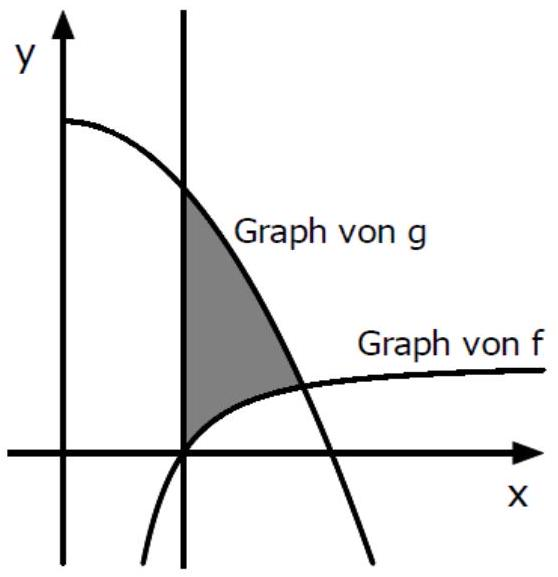
\includegraphics[max width=\textwidth, center]{2025_04_24_9018682670544743588fg-2}

\section*{Aufgabe 2: (1 VP und 1,5 VP)}
Betrachtet werden die in $\mathbb{R}$ definierten Funktionen $f$ und $F$, wobei $F$ eine Stammfunktion von $f$ ist. Die Abbildung in der Anlage zeigt den Graphen $G_{F}$ von $F$.\\
a) Bestimmen Sie den Wert des Integrals $\int_{1}^{7} f(x) d x$.\\
b) Bestimmen Sie den Funktionswert von $f$ an der Stelle $x_{0}=1$.

Veranschaulichen Sie Ihr Vorgehen in der Abbildung.

\section*{Aufgabe 3: (0,5 VP und 2 VP)}
Gegeben sind die in $\mathbb{R}$ definierten ganzrationalen Funktionen $f_{k}$ mit $f_{k}(x)=x^{4}+(2-k) \cdot x^{3}-k \cdot x^{2}$ mit $k \in \mathbb{R}$.\\
a) Begründen Sie, dass der Graph von $f_{2}$ symmetrisch bezüglich der y-Achse ist.\\
b) Es gibt einen Wert von $k$, für den $x_{w}=1$ eine Wendestelle von $f_{k}$ ist.

Berechnen Sie diesen Wert von k .

\section*{Aufgabe 4: (2,5 VP)}
Ermitteln Sie eine Gleichung derjenigen quadratischen Funktion g, die die beiden folgenden Eigenschaften hat:

\begin{itemize}
  \item Der Graph von g schneidet die Gerade mit der Gleichung $y=\frac{1}{4} x+1$ im Punkt $\mathrm{P}(0 \mid 1)$ unter einem rechten Winkel.
  \item Die $x$ - und die y-Koordinate des Extrempunkts des Graphen von g stimmen überein.
\end{itemize}

\section*{Aufgabe 5: (0,5 VP und 2 VP)}
Gegeben sind die Gerade $g: \vec{x}=\left(\begin{array}{l}7 \\ 3 \\ 3\end{array}\right)+r \cdot\left(\begin{array}{c}3 \\ 0 \\ -1\end{array}\right), r \in \mathbb{R}$, und die Ebene E: $3 x_{1}-x_{3}=-2$.\\
a) Begründen Sie, dass g orthogonal zu E ist.\\
b) Die Gerade $h: \vec{x}=\left(\begin{array}{l}7 \\ 3 \\ 3\end{array}\right)+s \cdot\left(\begin{array}{l}1 \\ 2 \\ 3\end{array}\right), s \in \mathbb{R}$, hat mit $E$ keinen gemeinsamen Punkt.

Es gibt Geraden, die in E liegen und parallel zu h verlaufen. Bestimmen Sie eine Gleichung derjenigen dieser Geraden, die von $h$ den kleinsten Abstand hat.

\section*{Aufgabe 6: (1,5 VP und 1 VP)}
Wird der Punkt $\mathrm{P}(1|2| 3)$ an der Ebene E gespiegelt, so ergibt sich der Punkt Q(7|2|11).\\
a) Bestimmen Sie eine Gleichung von E in Koordinatenform.\\
b) Auf der Geraden durch $P$ und $Q$ liegen die Punkte $R$ und $S$ symmetrisch bezüglich E; dabei liegt R bezüglich E auf der gleichen Seite wie P.\\
Der Abstand von $R$ und $S$ ist doppelt so groß wie der Abstand von $P$ und $Q$. Bestimmen Sie die Koordinaten von R.

\section*{Aufgabe 7: (1,5 VP und 1 VP)}
Die Zufallsgröße $X$ ist binomialverteilt mit den Parametern $n$ und $p=0,5$. Sie hat den Erwartungswert $\mu=18$.\\
a) Bestimmen Sie den Wert von $n$ und die Standardabweichung von $X$.\\
b) Entscheiden Sie, ob $\mathrm{P}(\mathrm{X}=14)<\mathrm{P}(\mathrm{X}=22)$ ist, und begründen Sie Ihre Entscheidung.

\section*{Aufgabe 8: (2,5 VP)}
Für ein Spiel wird ein Behälter mit 100 Kugeln gefüllt. Dafür stehen rote und blaue Kugeln zur Verfügung. Vor jedem Spiel legt der Spieler die Anzahl der blauen Kugeln im Behälter fest. Anschließend wird dem Behälter eine Kugel zufällig entnommen. Ist diese Kugel rot, so wird dem Spieler die festgelegte Anzahl blauer Kugeln in Cent ausgezahlt; ist die Kugel blau, so beträgt die Auszahlung 10 Cent. Ermitteln Sie, wie der Spieler die Anzahl blauer Kugeln für ein Spiel festlegen muss, damit der Erwartungswert der Auszahlung möglichst groß ist.

\section*{Abbildung zu Aufgabe 2 (Pflichtteil Aufgabensatz 1)\\}
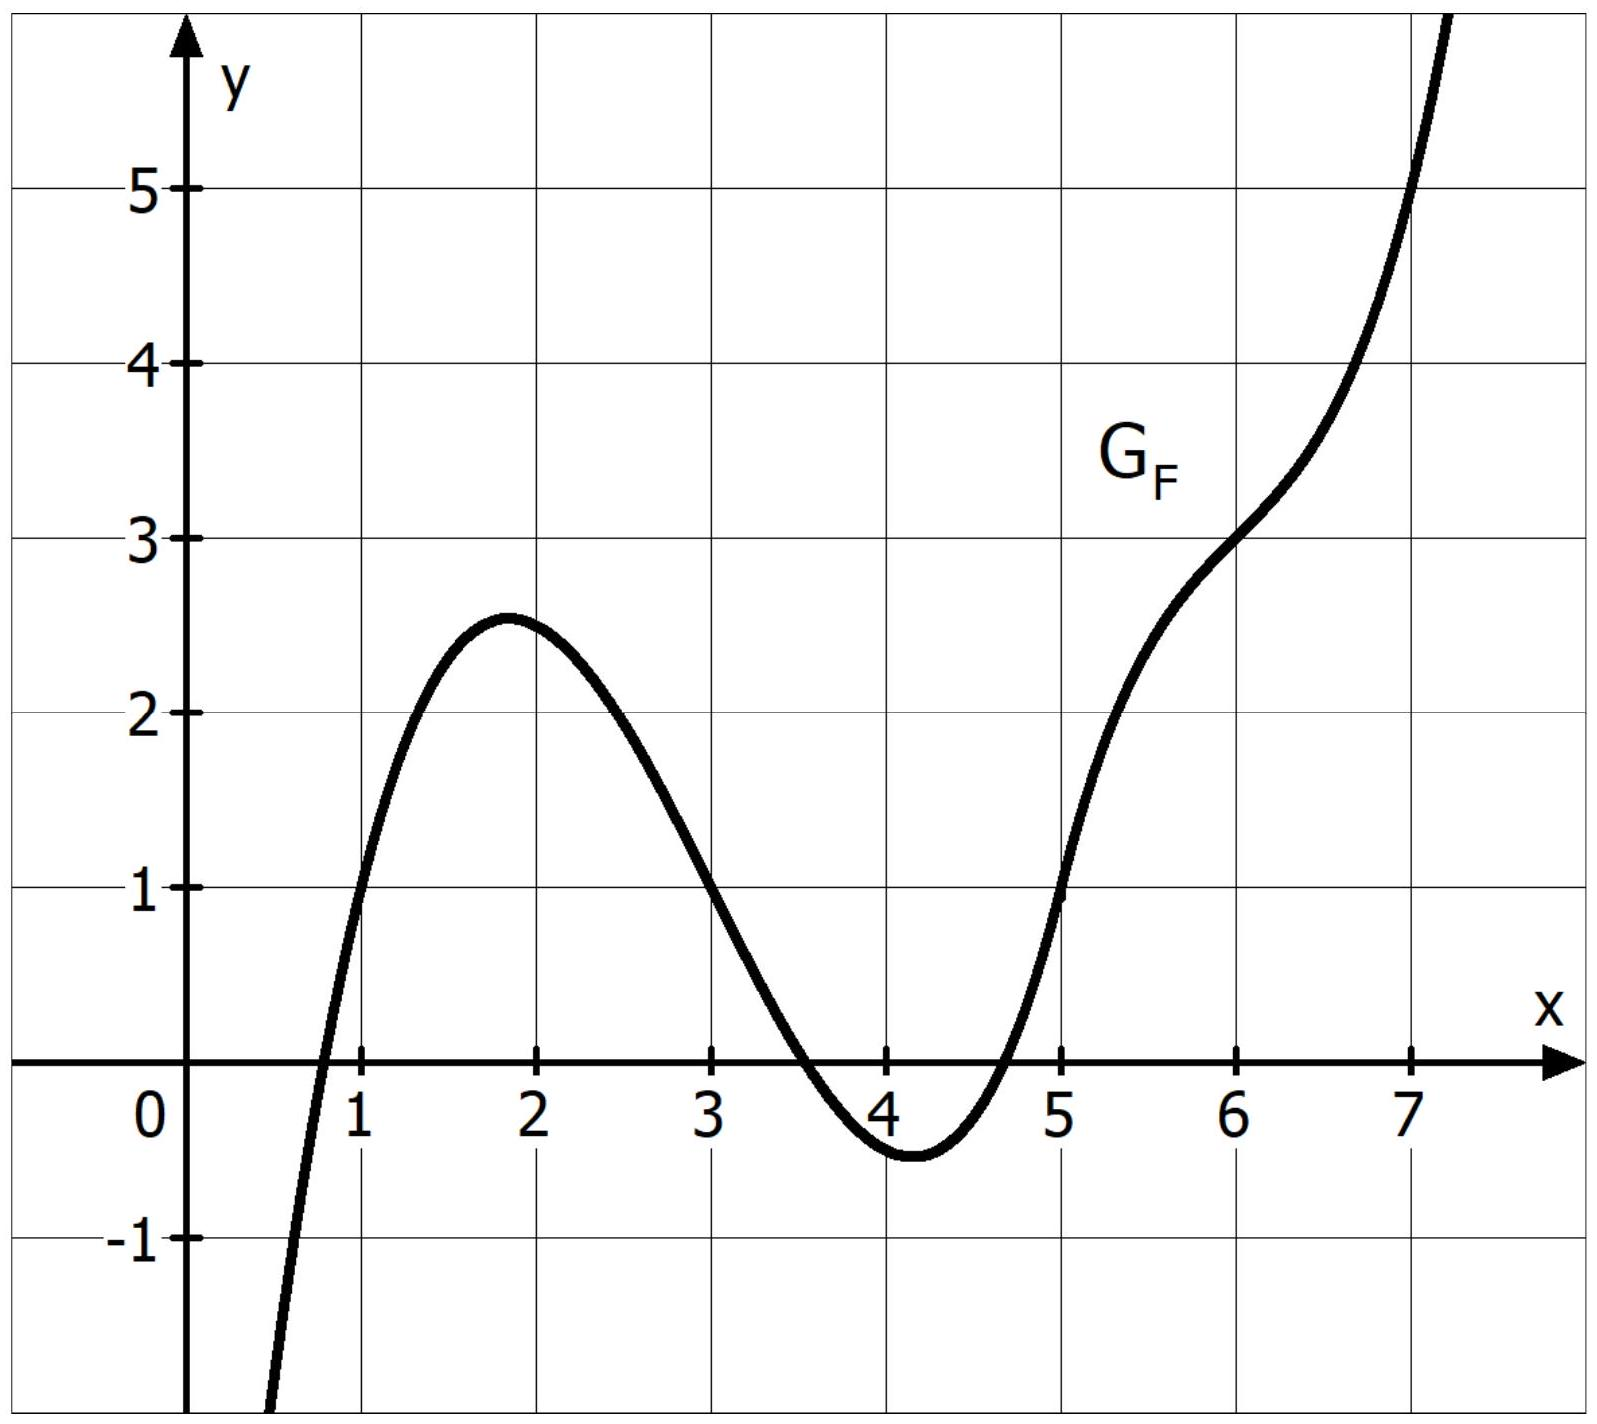
\includegraphics[max width=\textwidth, center]{2025_04_24_9018682670544743588fg-4}

\section*{Lösungen}
\section*{Aufgabe 1:}
a) Nachweis, dass sich die Schaubilder an der Stelle $x=2$ schneiden:

Es gilt $f(2)=4-\frac{4}{2^{2}}=3$ und $g(2)=15-3 \cdot 2^{2}=15-12=3$.\\
Da $f(2)=g(2)$ ist, schneiden sich die Schaubilder an der Stelle $x=2$.\\
b) Berechnung des Flächeninhalts:

$$
\begin{aligned}
A & =\int_{1}^{2}(g(x)-f(x)) d x=\int_{1}^{2}\left(15-3 x^{2}-\left(4-\frac{4}{x^{2}}\right)\right) d x=\int_{1}^{2}\left(11-3 x^{2}+4 x^{-2}\right) d x \\
& =\left[11 x-x^{3}-4 x^{-1}\right]_{1}^{2}=\left[11 x-x^{3}-\frac{4}{x}\right]_{1}^{2}=22-8-2-(11-1-4)=6 \text { FE }
\end{aligned}
$$

\section*{Aufgabe 2:}
a) $\int_{1}^{7} f(x) d x=[F(x)]_{1}^{7}=F(7)-F(1)=5-1=4$\\
b) $f(1)=F^{\prime}(1) \approx 4$ (Steigung der Tangente an das Schaubild von $F$ )\\

\section*{Aufgabe 3:}
Es gilt $f_{k}(x)=x^{4}+(2-k) \cdot x^{3}-k \cdot x^{2}$.\\
a) Für $k=2$ lautet er Funktionsterm $f_{2}(x)=x^{4}-2 \cdot x^{2}$.

Da der Funktionsterm nur Potenzen mit geraden Hochzahlen (Exponenten).\\
Somit ist der Graph von $f_{2}$ symmetrisch zur y-Achse.\\
b) Notwendige Bedingung für eine Wendestelle: $f_{k}{ }^{\prime \prime}(x)=0$\\
$f_{k}^{\prime}(x)=4 x^{3}+3 \cdot(2-k) \cdot x^{2}-2 k \cdot x$\\
$f_{k}^{\prime \prime}(x)=12 x^{2}+6 \cdot(2-k) \cdot x-2 k$

Bedingung: $\mathrm{f}_{\mathrm{k}}{ }^{\prime \prime}(1)=0: 12+6(2-\mathrm{k}) \cdot 1-2 \mathrm{k}=0 \Leftrightarrow 24-8 \mathrm{k}=0 \Leftrightarrow \mathrm{k}=3$\\
Für $\mathrm{k}=3$ ist die Bedingung erfüllt.\\
Hinweis:\\
Da in der Aufgabe vorgegeben ist, dass eine Wendestelle existiert, muss die Bedingung $\mathrm{f}_{\mathrm{k}}^{\prime \prime \prime}(1) \neq 0$ nicht geprüft werden.

\section*{Aufgabe 4:}
Ansatz für die Funktionsgleichung: $g(x)=a x^{2}+b x+c$\\
Es gilt $\mathrm{g}^{\prime}(\mathrm{x})=2 \mathrm{ax}+\mathrm{b}$.\\
$P(0 \mid 1)$ liegt auf dem Schaubild: $g(0)=1: \quad c=1$\\
senkrechter Schnitt:\\
Die gegeben Gerade hat die Steigung $\frac{1}{4}$, damit hat die Tangente an das Schaubild von $h$ im Punkt $P$ die Steigung $m=-\frac{1}{1 / 4}=-4$.\\
Bedingung: $g^{\prime}(0)=-4: b=-4$\\
Zwischenergebnis der Funktionsgleichung: $g(x)=a x^{2}-4 x+1$\\
Übereinstimmung der $x$ - und $y$-Koordinate des Extrempunktes:\\
Berechnung der Extremstelle von h: $\mathrm{g}^{\prime}(\mathrm{x})=0$\\
$g^{\prime}(x)=2 a x-4$\\
$2 \mathrm{ax}-4=0 \Leftrightarrow \mathrm{x}=\frac{4}{2 \mathrm{a}}=\frac{2}{\mathrm{a}}$

Nun soll gelten: $g\left(\frac{2}{a}\right)=\frac{2}{a}: a \cdot\left(\frac{2}{a}\right)^{2}-4 \cdot \frac{2}{a}+1=\frac{2}{a}$

$$
\begin{aligned}
& a \cdot \frac{4}{a^{2}}-\frac{8}{a}+1=\frac{2}{a} \\
& \Leftrightarrow \frac{4}{a}-\frac{8}{a}+1=\frac{2}{a} \\
& \Leftrightarrow 1=\frac{6}{a} \\
& \Leftrightarrow a=6
\end{aligned}
$$

Funktionsgleichung: $g(x)=6 x^{2}-4 x+1$

\section*{Aufgabe 5:}
a) $g$ ist orthogonal zu $E$, da der Richtungsvektor $\left(\begin{array}{c}3 \\ 0 \\ -1\end{array}\right)$ ein Normalenvektor von $E$ ist.\\
b) 
Die Gerade g ist orthogonal zu E und enthält den Punkt $P(7|3| 3)$ der Gerade $h$.\\
Die gesuchte Gerade auf E, die zu h den kleinsten Abstand besitzt ist parallel zu h und verläuft durch den Schnittpunkt S der Gerade g und Ebene E.

Schnittpunktberechnung von $g$ und E :\\
$3 \cdot(7+3 r)-(3-r)=-2$\\
$\Leftrightarrow 21+9 r-3+r=-2$\\
$\Leftrightarrow 10 r=-20 \Leftrightarrow r=-2$\\
Einsetzen von $r=-2$ in $g$ ergibt den Schnittpunkt $S(1|3| 5)$.\\
Die Gleichung der gesuchten Geraden lautet $\vec{x}=\left(\begin{array}{l}1 \\ 3 \\ 5\end{array}\right)+t \cdot\left(\begin{array}{l}1 \\ 2 \\ 3\end{array}\right)$.

\section*{Aufgabe 6:}
a) Die gesuchte Ebene E besitzt den Normalenvektor $\overrightarrow{\mathrm{PQ}}=\left(\begin{array}{l}6 \\ 0 \\ 8\end{array}\right)$.

Der Mittelpunkt M der Strecke $\overline{\mathrm{PQ}}$ liegt ebenfalls auf E .\\
Koordinaten von $M$ : $M\left(\frac{1+7}{2}\left|\frac{2+2}{2}\right| \frac{3+11}{2}\right)$, also $M(4|2| 7)$.\\
Ansatz für die Koordinatengleichung: $6 \mathrm{x}_{1}+8 \mathrm{x}_{3}=\mathrm{d}$\\
Einsetzen von $\mathrm{M}(4|2| 7): 6 \cdot 4+8 \cdot 7=\mathrm{d}$\\
Koordinatengleichung: $6 x_{1}+8 x_{3}=80$ bzw. vereinfacht $3 x_{1}+4 x_{3}=40$\\
b) 
Koordinaten von R :\\
$\overrightarrow{\mathrm{OR}}=\overrightarrow{\mathrm{OM}}+2 \cdot \overrightarrow{\mathrm{MP}}=\left(\begin{array}{l}4 \\ 2 \\ 7\end{array}\right)+2 \cdot\left(\begin{array}{c}-3 \\ 0 \\ -4\end{array}\right)=\left(\begin{array}{c}-2 \\ 2 \\ -1\end{array}\right)$\\
Der Punkt $R$ hat die Koordinaten $R(-2|2|-1)$.

\section*{Aufgabe 7:}
a) Es gilt $\mu=\mathrm{n} \cdot \mathrm{p}$.\\
$18=n \cdot 0,5 \Leftrightarrow n=36$\\
Standardabweichung: $\sigma=\sqrt{n \cdot p \cdot(1-p)}=\sqrt{36 \cdot 0,5 \cdot 0,5}=\sqrt{9}=3$\\
b) Da $p=0,5$ ist, ist die Verteilung symmetrisch zum Erwartungswert.

Da die Werte 14 und 22 gleich weit vom Erwartungswert entfernt sind, gilt $P(X=14)=P(X=22)$.\\
Die Aussage ist falsch.

\section*{Aufgabe 8:}
Die Anzahl der blauen Kugeln sei x .\\
Die Anzahl der roten Kugeln ist dann 100-x.\\
Es gilt: $P($ blau $)=\frac{x}{100}$ und $P($ rot $)=\frac{100-x}{100}$.\\
Die Zufallsgröße X gebe den Auszahlungsbetrag in Cent an.\\
Es gilt: $P(X=x)=\frac{100-x}{100}$ und $P(X=10)=\frac{x}{100}$.\\
Erwartungswert von X :\\
$E(X)=x \cdot \frac{100-x}{100}+10 \cdot \frac{x}{100}=\frac{1}{100} \cdot\left(100 x-x^{2}+10 x\right)=0,01 \cdot\left(110 x-x^{2}\right)$\\
Gesucht ist das Maximum der Funktion $f(x)=0,01 \cdot\left(110 x-x^{2}\right)$\\
$f^{\prime}(x)=0,01 \cdot(110-2 x)$\\
$f^{\prime}(x)=0: 110-2 x=0 \Leftrightarrow x=55$\\
Da das Schaubild von $f$ eine nach unten geöffnete Parabel ist, muss bei $x=55$ ein Maximum existieren.\\
Der Spieler muss sich für 55 blaue Kugeln entscheiden.


\end{document}